\documentclass[t]{article}
\usepackage[english]{babel}
\usepackage[utf8]{inputenc}
%\usepackage{beamerthemeshadow}
\usepackage{amsmath} 
\usepackage{amssymb} 
\usepackage{caption} 
\usepackage{subcaption} 
\usepackage{listings}
\usepackage{tabularx}
\usepackage{listings}
\usepackage{color}
\usepackage{xcolor}
\usepackage{booktabs}


\definecolor{mygreen}{rgb}{0,0.6,0}
\definecolor{mygray}{rgb}{0.9,0.9,0.9}
\definecolor{mymauve}{rgb}{0.58,0,0.82}
\lstset{ %
  backgroundcolor=\color{mygray},   % choose the background color; you must add \usepackage{color} or \usepackage{xcolor}
  basicstyle=\footnotesize\ttfamily,        % the size of the fonts that are used for the code
  breakatwhitespace=false,         % sets if automatic breaks should only happen at whitespace
  breaklines=true,                 % sets automatic line breaking
  captionpos=b,                    % sets the caption-position to bottom
  commentstyle=\color{mygreen},    % comment style
  deletekeywords={...},            % if you want to delete keywords from the given language
  escapeinside={\%*}{*)},          % if you want to add LaTeX within your code
  extendedchars=true,              % lets you use non-ASCII characters; for 8-bits encodings only, does not work with UTF-8
  frame=none,	                   % adds a frame around the code
  keepspaces=true,                 % keeps spaces in text, useful for keeping indentation of code (possibly needs columns=flexible)
  keywordstyle=\color{black},       % keyword style
  language=bash,                    % the language of the code
  otherkeywords={*,...},           % if you want to add more keywords to the set
  numbers=left,                    % where to put the line-numbers; possible values are (none, left, right)
  numbersep=5pt,                   % how far the line-numbers are from the code
  numberstyle=\tiny\color{mygray}, % the style that is used for the line-numbers
  rulecolor=\color{black},         % if not set, the frame-color may be changed on line-breaks within not-black text (e.g. comments (green here))
  showspaces=false,                % show spaces everywhere adding particular underscores; it overrides 'showstringspaces'
  showstringspaces=false,          % underline spaces within strings only
  showtabs=false,                  % show tabs within strings adding particular underscores
  stepnumber=0,                    % the step between two line-numbers. If it's 1, each line will be numbered
  stringstyle=\color{mymauve},     % string literal style
  tabsize=2,	                   % sets default tabsize to 2 spaces
  title=\lstname                   % show the filename of files included with \lstinputlisting; also try caption instead of title
}
\usepackage{textcomp}
\usepackage{soul}
\usepackage{color}
\usepackage{hyperref}
\title{Building {\tt c++} code with {\tt JMakefile}}
\author{}
\date{\today}
\usepackage{lipsum}
\usepackage{graphicx}
\textwidth = 420pt
\marginparwidth = 0pt
\oddsidemargin = 31pt
\begin{document}

\maketitle
\begin{abstract}
This note contains a brief description of the implementation of the {\tt make} process within {\tt Jpp}. Examples of how to use the {\tt Makefiles} included in {\tt Jpp} to compile a {\tt c++} project are given.
\end{abstract}

\section{{\tt Jpp} makefiles}
The makefiles included in {\tt Jpp} can be used for several purposes. Besides compiling the {\tt Jpp} source code, one can build {\tt .pdf} documents from {\tt .tex} files, they can be used to build {\tt c++} projects including the compilation of dynamic libraries, and one can also convert libreoffice documents to {\tt .pdf} files. The instructions and variabes that {\tt make} will follow are distributed in several {\tt makefiles} organised according to the structure shown in figure \ref{fig:JMake_structure}.
\begin{figure}[h]
\center
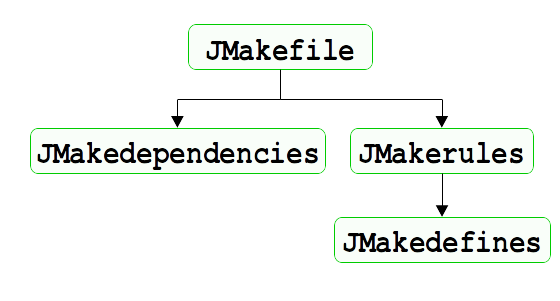
\includegraphics[width=8cm]{./plots/JMake_structure}
\caption{Structure of the {\tt jpp Makefiles}. {\tt JMakefile} includes {\tt JMakerules} and {\tt JMakedependencies}, the former of which includes {\tt JMakedefines}.}\label{fig:JMake_structure}
\end{figure}
If one takes a look at these {\tt makefiles}, they look as follows. 

\begin{lstlisting}
#JMakefile
------------------------------------
include $(JPP_DIR)/JMakerules
include $(JPP_DIR)/JMakedependencies
\end{lstlisting}
{\tt JMakefile} is rather simple. It only includes {\tt JMakerules} and {\tt JMakedependencies}. {\tt JMakerules} is structured as follows,
\begin{lstlisting}
#JMakerules
------------------------------------
include $(JPP_DIR)/JMakedefines
{
	definition of pattern rules
}
{
	definition of file lists and assignation of default values
}
\end{lstlisting}
where 

\begin{lstlisting}
#JMakedefines
------------------------------------
{
	definition of auxiliary functions
}
{
	definition of global variables
}
\end{lstlisting}
Finally, {\tt JMakedependencies} has the following structure

\begin{lstlisting}
#JMakedependencies
------------------------------------
{
	definition of phony targets and top level rules for lists of flies
}
{
	inclussion of dependency files generated by the compiler
}
\end{lstlisting}
%Therefore, the information contained in the {\tt Jpp} makefiles can be grouped into the following categories: definition of auxiliary functions, definition of variables, definition of pattern rules for single files, definition of file lists, definition of phony targets and top-level rules for lists of files, and inclussion of the dependency files generated by the {\tt c++} compiler.
In what follows, a description of the most relevant functions, variables and rules needed to compile a {\tt c++} project is given. 
\subsection{Auxiliary functions}
The functions defined in {\tt JMakedefines} are mainly functions for the treatment of strings of characters. Among these functions one can find for instance the {\tt insert} function, which inserts a path in a string of paths and which can be used to update environmental variables such as {\tt LD$\_$LIBRARY$\_$PATH} or {\tt PATH}. Another interesting function is the {\tt binary} function, which given a list of {\tt c++} source code files (with {\tt .cc} extension) finds which files contain the {\tt int main} method and returns a list with the corresponding binary file names (ie, the same file names but without the {\tt .cc} extension).  
\subsection{Global variables}
Variables related to the multiple actions that can be carried out by the {\tt Jpp makefiles} are defined inside {\tt JMakedefines}. Some of them are mentioned in the following sections, and a brief description of other which are relevant for the compilation of {\tt c++} projects is given in the appendix\ref{sec:appendix_a}
\subsection{Pattern rules}
Several pattern rules are included in {\tt JMakerules} that implement the compilation, linking and document generation. The pattern rules for compiling {\tt c++} source code files into object files and for linking of object files into binary files are shown below 

\begin{lstlisting}
#Compilation pattern rule
------------------------------------
%.o: %.cc %.d
	$(CXX) $(CXXFLAGS) $(CPPFLAGS) -c -o $@ $<

#Linking pattern rule
------------------------------------
%: %.o
	$(CXX) $(LDFLAGS) -o $@ $^ $(LOADLIBES)

\end{lstlisting}
{\tt CXX = g++} is the compiler and {\tt CXXFLAGS} and {\tt CPPFLAGS } are lists of options that can be passed to the compiler and the preprocessor respectively. {\tt CXXFLAGS} should  include the list of paths pointing to the location of the {\tt .hh} files included in the {\tt c++} source code files that are compiled. {\tt LDFLAGS} is a list of paths pointing to the location of external libraries needed to link several objects into an executable, and {\tt LOADLIBES} is a list of external libraries. These variables are set to some default values by {\tt JMakedefines} which are listed on \ref{sec:appendix_a}.

\subsection{Native and Public file lists}  
{\tt JMakerules} includes the definition of {\tt NATIVE$\_$} and {\tt PUBLIC$\_$} variables to store file lists. The native file lists are reserved for those files existing in the directory from which {\tt JMakefile} is called (or "current directory"). The variable {\tt NATIVE$\_$SRCS} will be filled with a list of all the files with {\tt .cc} extension, the variable {\tt NATIVE$\_$OBJS} will contain the list of corresponding object file names, and {\tt NATIVE$\_$BIN} will contain a list of binary file names corresponding to every source file that contains a {\tt main} function (this is achieved thanks to the {\tt binary} function described above). In addition, {\tt NATIVE$\_$SCRIPTS} conatins a lists of {\tt .sh} files and {\tt NATIVE$\_$DOCS} a list of {\tt .tex, .docx} and {\tt .pptx} files. If the current directory is a sub-directory of {\tt $\$$JPP$\_$DIR/software}, then the lists of files are stored in the public variables ({\tt PUBLIC$\_$SRCS}, {\tt PUBLIC$\_$BIN}...etc).

\subsection{Phony targets}   
{\tt JMakedependencies} includes the declaration of several phony targets. Among those, the most relevant are {\tt default, all, install} and {\tt clean}. The default target (ie the first target appearing in the makefile structure, which is the one that will be remade if no target is specified when launching make) is {\tt default}, which in turn has {\tt all} and {\tt install} as prerequisites. The prerequisites of {\tt all} are the {\tt NATIVE} lists, and the prerequisites of {\tt install} are the {\tt PUBLIC} lists. Therefore, by default all the files in the current directory are remade according to the corresponding pattern rules. 

\section{Using {\tt JMakefile} to build a {\tt c++} project}
Since {\tt JMakefile} implements the majority of the functions and rules needed by make to compile and link {\tt c++} code, using it to build one's own project is rather straightforward. One just have to create a {\tt Makefile} that includes {\tt JMakefile}, where the compilation and linking variables are accordingly updated with the desired library paths, include paths and external libraries. By default, {\tt JMakefile} doesn't know which object files need to be linked into a binary file. If a binary file is obtained from the compilation and linking of more than one source code file, the user should specify this information in the {\tt Makefile}. This is simply done by writing an explicit rule with the final binary file as a target, the object files to be linked as prerequisites. {\tt JMakefile} will use the appropriate pattern rules to generate the object files and the final binary file. A typical {\tt Makefile} would be like this:

\begin{lstlisting}
#My Makefile
------------------------------------
include $(JPP_DIR)/JMakefile

LDFLAGS += -L/path/...
CXXFLAGS += -I/path/...
LOADLIBES += -l...

main: main.o lib1.o lib2.o ...etc
\end{lstlisting}

The \textbf{first example} included with this document consists on three {\tt c++} files plus a {\tt Makefile}. The {\tt c++} files consist on {\tt JMain.cc}, where the main method calls the {\tt lib} function that is defined in {\tt JLib.hh} and implemented in {\tt JLib.cc}. The {\tt Makefile} to build the {\tt JMain} binary file is simply 
\begin{lstlisting}
#My Makefile
------------------------------------
include $(JPP_DIR)/JMakefile
JMain: JMain.o JLib.o
\end{lstlisting}

The \textbf{second example} compiles the same binary file as in the first example, but following a different strategy that better suits with the {\tt Jpp} philosophy. This is, defining and implementing the classes and functions in a single include file. In this case the project consists only on two {\tt c++} files plus the {\tt Makefile}. The diference with respect to the previous example is that in this case the {\tt JLib.cc} file doesn't exist, and both the definition and implementation of the {\tt lib} function is done inside {\tt JLib.hh}. In this case the rules included in {\tt JMakefile} are enough to build the only the only file to be compiled is {JMain.cc}, and the {\tt Makefile} can be simplified to a single line. 
\newpage
\begin{lstlisting}
#My Makefile
------------------------------------
include $(JPP_DIR)/JMakefile
\end{lstlisting}

\section*{Appendix A: relevant variables defined in {\tt JMakefile}}
Here, a list of variables defined or updated in {\tt JMakedefines} that one may need to use in an owns {\tt Makefile} is given. 
\subsection*{Environmental variables}
The envionrmental variables {\tt LD$\_$LIBRARY$\_$PATH} and {\tt PATH} are updated by {\tt JMakedefines}:
\begin{itemize}
\item {\tt PATH}: The path {\tt $\$$ROOTSYS/bin} is appended to the {\tt PATH}
\item {\tt LD$\_$LIBRARY$\_$PATH}: The paths {\tt $\$$ROOTSYS/lib , JPP$\_$LIB} and {\tt AANET$\_$LIB} are appended to the {\tt LD$\_$LIBRARY$\_$PATH} 
\end{itemize}
\subsection*{Default {\tt g++} options}
The default values of the compiler variables mentioned above include the following libraries and paths
\begin{itemize}
\item {\tt CXXFLAGS} include the following paths pointing to include files: {\tt JPP$\_$INCLUDE, ROOTINCL, AANET$\_$INCLUDE(/evt /util), ANTARES$\_$INCLUDE}.
\item {\tt LDFLAGS} include the following paths pointing to external libraries: {\tt JPP$\_$LIB, AANET$\_$LIB, ANTARES$\_$LIB}.
\item {\tt LOADLIBES} includes by default {\tt JPP$\_$LIBS} and {\tt ROOTLIBS}
\end{itemize} 
see below for a description of these variables. 
\subsection*{{\tt Jpp} variables}
\begin{itemize}
\item {\tt JPP$\_$INCLUDE = $\$$JPP$\_$DIR/software}: Path to the location of {\tt Jpp} include files. 
\item {\tt JPP$\_$LIB = $\$$JPP$\_$DIR/$\$$SYSTEM/lib/}: Path to {\tt Jpp} libraries. Here, the {\tt SYSTEM = Linux} is another variable. The variables for different of these libraries are the following:
\begin{itemize}
\item {\tt JPP$\_$LIBS = -llang}
\item {\tt JDAQ$\_$LIBS = -lKM3NeTDAQROOT}
\item {\tt JDAQ$\_$CHSM = -lDAQ$\_$CHSM}
\item {\tt JTRIGGER$\_$LIBS = -ltriggerROOT}
\item {\tt JEVT$\_$LIBS = -levtROOT}
\item {\tt JAANET$\_$LIBS = -ljaanetROOT}
\item {\tt JMARKOV$\_$LIBS = -lmarkovROOT}
\end{itemize}
\end{itemize}
\subsection*{{\tt aanet} variables} 
\begin{itemize}
\item {\tt AANET$\_$INCLUDE = $\$$JPP$\_$DIR/externals/aanet/}: Path to the location of aanet {\tt .hh} files. 
\item {\tt AANET$\_$LIB = $\$$JPP$\_$DIR/externals/aanet/}: Path to the aanet external libraries. The variable containing the libraries is
\begin{itemize}
\item {\tt AANET$\_$LIBS = -laa}
\end{itemize} 
\end{itemize}

\subsection*{Database}
\begin{itemize}
\item {\tt JDB$\_$INCLUDE = $\$$JPP$\_$DIR/externals/dbclient/include} 
\item {\tt JDB$\_$LIB = $\$$JPP$\_$DIR/externals/dbclient/lib}
\begin{itemize}
\item {\tt JDB$\_$LIBS = -lKM3NeTDBClient}
\end{itemize} 
\end{itemize}

\subsection*{Antares}
\begin{itemize}
\item {\tt ANTARES$\_$INCLUDE = $\$$JPP$\_$DIR/externals/} 
\item {\tt JDB$\_$LIB = $\$$JPP$\_$DIR/externals/antares-dataformat/}
\begin{itemize}
\item {\tt ANTARES$\_$LIBS = -lAntaresDAQROOT}
\end{itemize} 
\end{itemize}

\subsection*{ROOT}
\begin{itemize}
\item {\tt ROOTLIBS       =  $\$${ROOTSYS}/bin/root-config --libs}
\item {\tt ROOTGLIBS      = $\$${ROOTSYS}/bin/root-config --glibs}
\item {\tt ROOTINCL       = $\$${ROOTSYS}/bin/root-config --cflags}
\item {\tt ROOTCINTFLAGS  = -I$\$$(JPP$\_$INCLUDE) -DNAMESPACE=ANTARES / KM3NeT}

\end{itemize}
%
%\begin{thebibliography}{1}
%\end{thebibliography}

\end{document}
